\documentclass[11pt]{article}
\usepackage[left=2cm,right=2cm,top=2cm,bottom=3cm]{geometry}
\usepackage{graphicx}
\usepackage{float}
\usepackage[spanish]{babel}
\usepackage{url}
\usepackage[american]{circuitikz}

\begin{document}

\title{Tarea 1\\Circuitos limitadores}
%\subtitle{Circuitos limitadores}
\author{Elementos Activos\\Dr.-Ing. Juan José Montero Rodríguez}
%\subject{Elementos Activos}
\maketitle

\section{Introducción}

Implemente en LTspice o Multisim el circuito limitador de la Figura \ref{limitador_circuito}. Este circuito se utiliza para convertir una forma de onda triangular de entrada a una señal de salida que es más suave, similar a una senoidal.


\begin{figure}[H]
    \centering    
    \begin{circuitikz}
        \draw (0,6) to[sV,l_=$V_{S}$] (0,0);
        \draw (0,6) to[R,l=$R_S$] (3,6);
        \draw (3,6) to[short,-o] (14,6);
        \draw (0,0) to[short] (14,0);
        \draw (14,6) node[right]{$V_{out}$};
        \draw (14,0) node[ground]{};
        \draw (3,6) to[D,l=$D_1$] (3,4);
        \draw (3,4) to[V,l=$V_1$] (3,2);
        \draw (3,2) to[R,l=$R_1$] (3,0);
        \draw (6,4) to[D,l_=$D_2$] (6,6);
        \draw (6,2) to[V,l_=$V_2$] (6,4);
        \draw (6,2) to[R,l=$R_2$] (6,0);
        \draw (9,6) to[D,l=$D_3$] (9,4);
        \draw (9,4) to[V,l=$V_3$] (9,2);
        \draw (9,2) to[short] (9,0);
        \draw (12,4) to[D,l_=$D_4$] (12,6);
        \draw (12,2) to[V,l_=$V_4$] (12,4);
        \draw (12,2) to[short] (12,0);
    \end{circuitikz}
    \caption{Circuito limitador.}
    \label{limitador_circuito}
\end{figure}

El circuito limitador deberá entregar una tensión de salida definida por la siguiente función:

\begin{figure}[H]
    \centering
    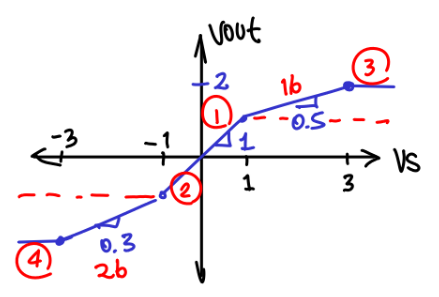
\includegraphics[width=0.5\textwidth]{limitador_1.png}
    \caption{Función de transferencia del circuito limitador}
    \label{limitador_transferencia}
\end{figure}

El objetivo de la tarea es simular la función de transferencia del circuito, y la respuesta transitoria.

\section{Procedimiento}

\subsection{Simulación con diodos ideales}

\subsubsection{Simulación de la función de transferencia}

\begin{enumerate}
    \item Cree un nuevo archivo de texto llamado \texttt{Dideal.mod} y agregue el siguiente código:

    \begin{verbatim}
        .model Dideal D(Ron=0.1n Roff=1G Vfwd=0.7)
    \end{verbatim}

    \item Cree un archivo de LTspice nuevo con nombre \texttt{limitador-ideal-dc.asc}.
    \item Construya el diagrama esquemático del limitador en LTspice.
    \item En el diagrama de LTspice, agregue un bloque de directiva Spice (Atajo: S) y dentro de este bloque coloque el siguiente texto:

    \begin{verbatim}
        .include Dideal.mod
    \end{verbatim}
    
    \item Haga clic derecho en la etiqueta de cada diodo y cambie el nombre del modelo a \texttt{Dideal}.
    \item Haga clic en el menú Simulate y luego en Edit Simulation Cmd.
    \item Dimensione los valores de los componentes de forma teórica y agregue los valores al diagrama.
    \item Configure una simulación de barrido de CD para obtener la curva de transferencia.
\end{enumerate}

\subsubsection{Simulación de la respuesta transitoria}

\begin{enumerate}
    \item Haga una copia del archivo y guárdelo como \texttt{limitador-ideal-tran.asc}.
    \item Cambie la fuente por una triangular.
    \item Haga clic en el menú Simulate y luego en Edit Simulation Cmd.
    \item Configure una simulación transitoria y simule un ciclo completo.
\end{enumerate}


\subsection{Simulación con diodos comerciales}

Para esta sección, el circuito debe utilizar diodos comerciales modelo 1N4004, que se pueden descargar desde la referencia \cite{onsemi4004}.

\begin{enumerate}
    \item Guarde el archivo del modelo del diodo como \texttt{1N4004.txt}.
    \item Haga una copia del archivo de LTspice ideal y guarde el archivo como \texttt{limitador-4004-dc.asc}.
    \item Modifique el archivo y cambie las etiquetas de los diodos por \texttt{1N4004}.
    \item Realice la simulación de la función de transferencia.
    \item Repita los pasos para obtener la forma de onda en la simulación transitoria.
\end{enumerate}


\section{Instrucciones de presentación}

Debe elaborar un reporte en formato IEEE donde incluya la teoría del circuito, el funcionamiento ideal esperado, el dimensionamiento de los componentes, el procedimiento de simulación ideal y con diodos comerciales, mostrando todos los pasos, y la comparación entre las simulaciones ideales y comerciales. Agregue una discusión, conclusiones y referencias.

La tarea se debe entregar a más tardar el viernes 20 de octubre antes de las 11:59 p.m. por medio del tecDigital. Debe entregar un único archivo ZIP con el documento en PDF y las simulaciones en el formato de LTspice. No se recibirán entregas tardías.

Puede desarrollar la tarea en forma individual o en grupos de hasta cuatro personas.


\section{Rúbrica de evaluación}

\bibliographystyle{unsrt}
\bibliography{refs}



\end{document}
